% pScientists typically have to seek out the aid of software developers in order to obtain configuration files that matched their specifications. This is currently being done manually by editing large JSON files which is both fragile as well as time-consuming for both parties involved.

The NeXus Constructor is a tool written with Qt for Python which allows scientists to create, edit and visualise NeXus files with minimal assistance. Such files can then be used for configuring the experiment control software in order to write real-time data. The layout of the NeXus Constructor interface consists of 

\begin{itemize}
\item Instrument View - A widget built with Qt3D constructs that draws the experiment components in 3D. As NeXus files can contain information about a component's geometry and any transformations that may have been applied to it, translating this into something Qt3D can understand is fairly simple.
\item Component List - A list of the components that have been created so far. 
\item NeXus File Layout - An illustration of the hierarchical NeXus structure. Can't be used to see the values of the individual fields, but can serve as a tool through which you can check that the data has a sensible arrangement.
\end{itemize} % Someone may not know what experiment control software does, what makes real-time data good, etc.

To add a component a user presses the "Add Component" button and goes through a set of steps to enter the relevant details of the component they wish to add. A number of basic checks are performed to see if this data is sensible, and in many cases restricting 

\begin{figure}
\caption{Screenshot of the NeXus Constructor}
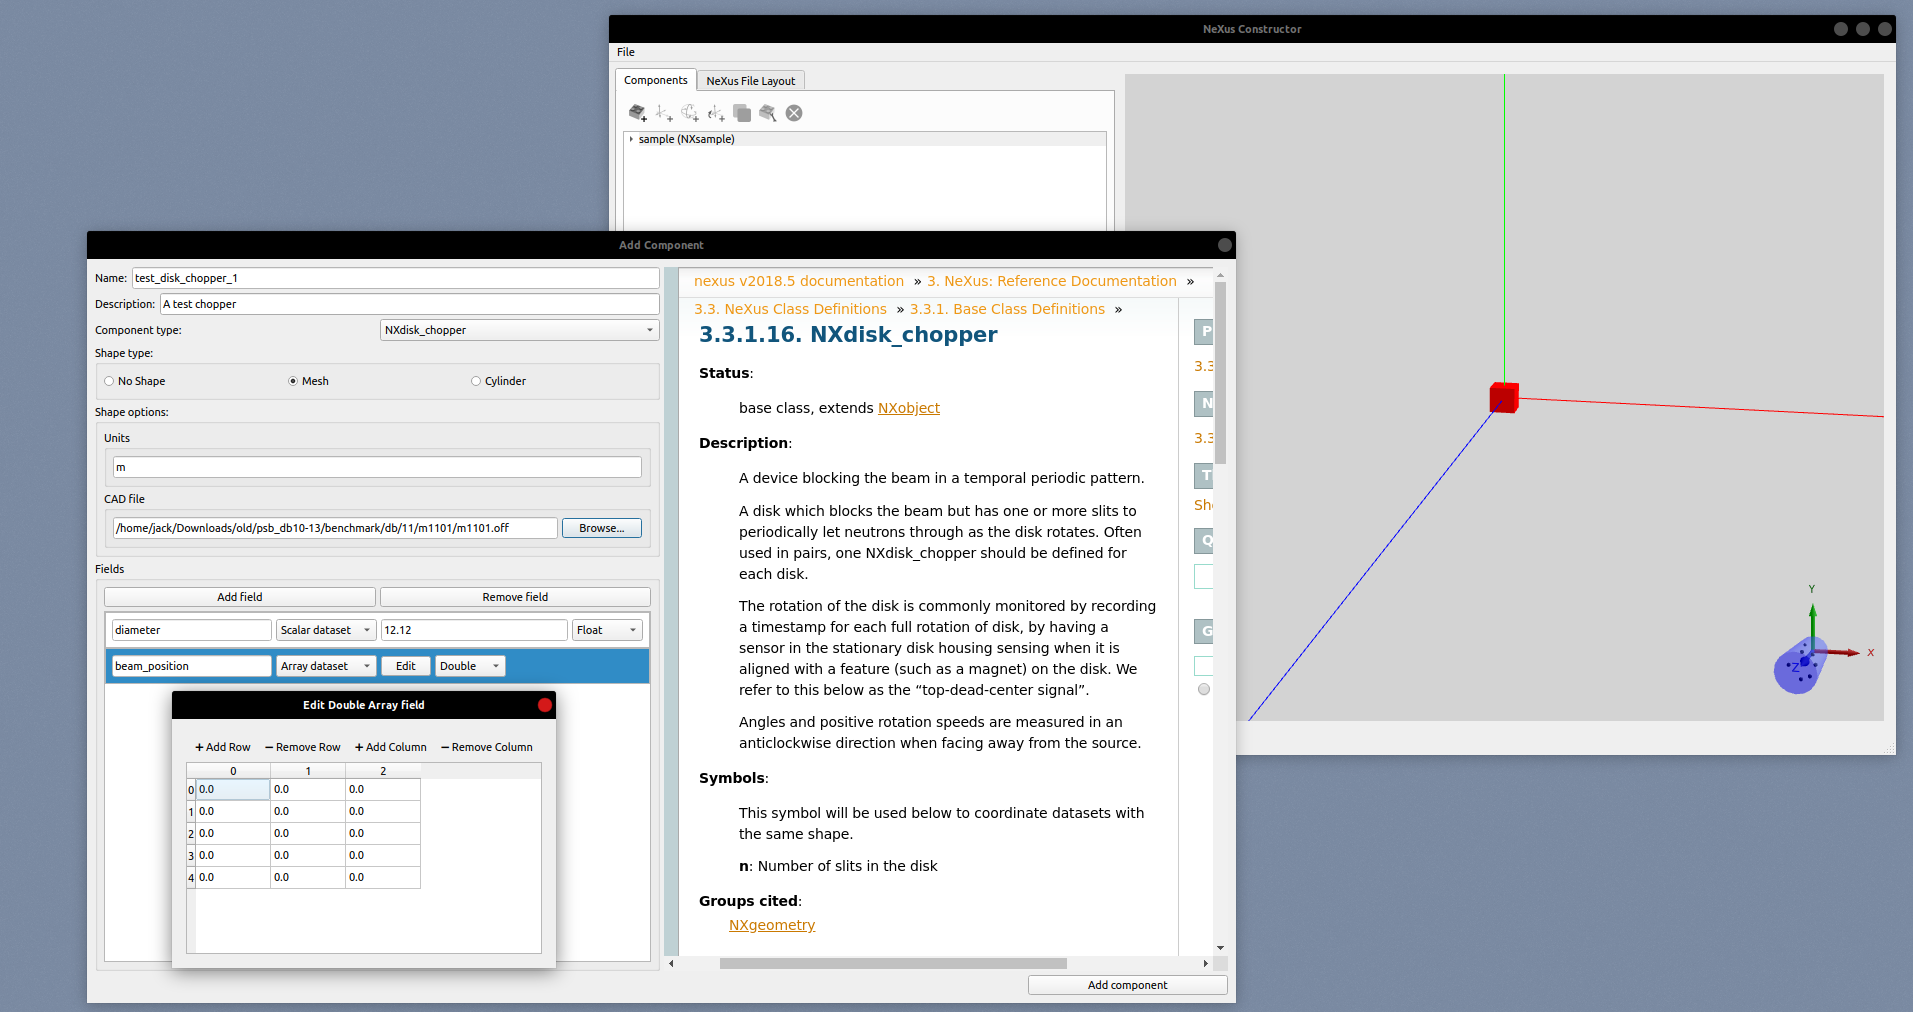
\includegraphics[width=\linewidth]{screenshot.png}
\end{figure}

The screenshot shows the main window of the NeXus Constructor and its "Add Component" dialog which allows users to add extra data in a NeXus file that describes the components that were present in an experiment.




